\documentclass[tikz,border=6pt]{standalone}
\usepackage{pgfplots}
\pgfplotsset{compat=1.18}
\begin{document}
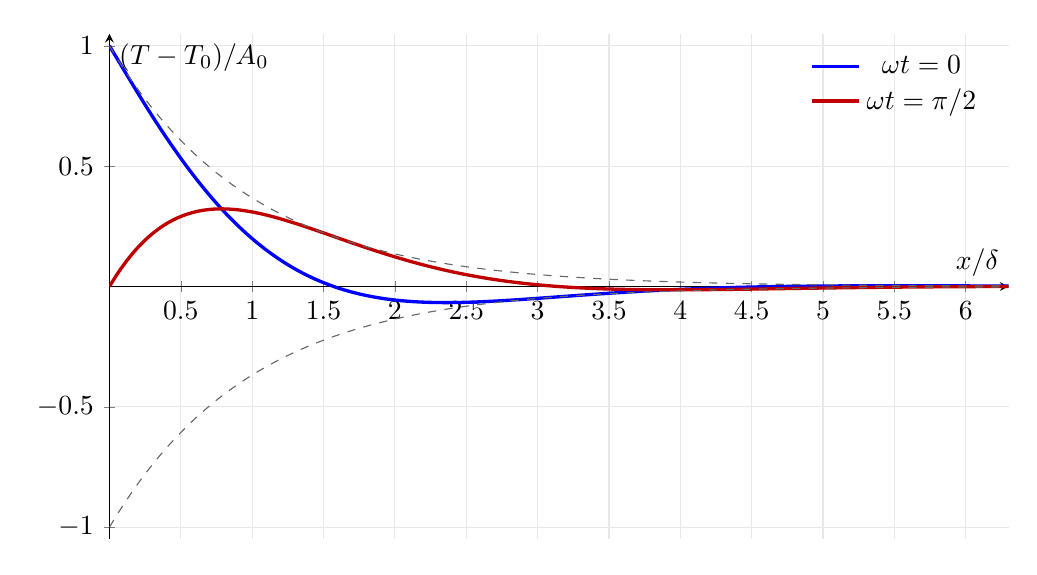
\begin{tikzpicture}
\begin{axis}[
 width=13cm,height=8cm,axis lines=middle,
 xlabel={$x/\delta$},ylabel={$(T-T_0)/A_0$},
 xmin=0,xmax=6.3,ymin=-1.05,ymax=1.05,
 samples=280,domain=0:6.3,
 legend style={draw=none,fill=none,at={(.98,.98)},anchor=north east},
 grid=major,grid style={gray!18}]
% delta=sqrt(2 alpha/omega); theta=exp(-x/delta)cos(omega t-x/delta).
\addplot[very thick,blue] {exp(-x)*cos(deg(x))};
\addlegendentry{$\omega t=0$}
\addplot[very thick,red!75!black] {exp(-x)*cos(deg(pi/2-x))};
\addlegendentry{$\omega t=\pi/2$}
\addplot[dashed,black!60] {exp(-x)};
\addplot[dashed,black!60] {-exp(-x)};
\end{axis}
\end{tikzpicture}
\end{document}
